\section{Design}
\label{sec:design}

Our goal is to leverage hardware-software co-design to develop a container networking system with both high performance and compatibility with existing software.

Due to limited PCIe throughput, we leave the data plane on the CPU and only process control messages via programmable NIC (FPGA).
We use NIC as the center of coordination instead of a dedicated core, because the NIC has much more processing capacity than a CPU core~\cite{li2016clicknp}.
We design the NIC to support three sets of functions:
\begin{enumerate}
\item A most frequently used subset of BSD socket semantics;
\item A pair of request and event queues per container process;
\item Epoll-compatible event dispatch.
\end{enumerate}

\begin{figure}[t]
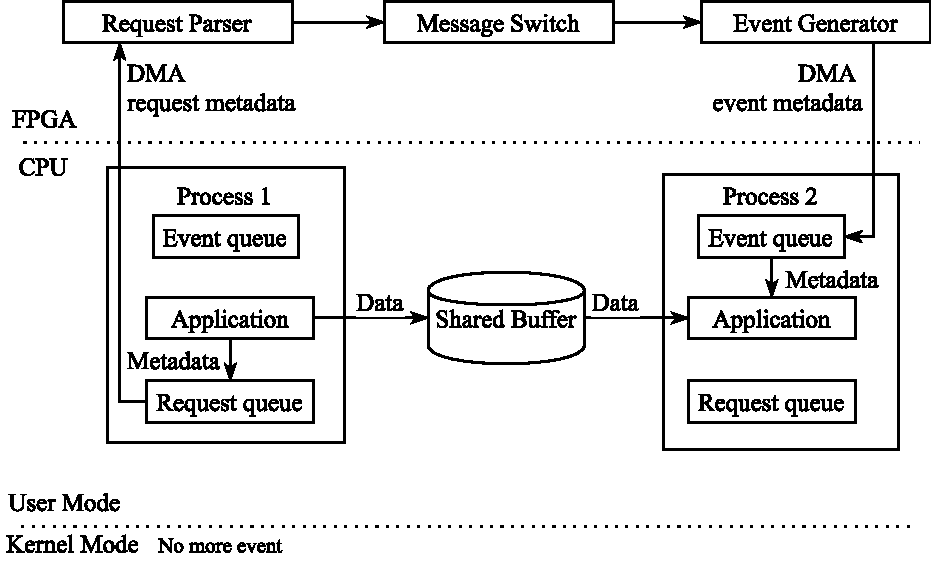
\includegraphics[width=0.47\textwidth]{ipc_msg_lifecycle_2.pdf}
\caption{Container Networking with Programmable NIC.}
\label{fig:arch}
\vspace{-0.2in}
\end{figure}

\textbf{Control plane on programmable NIC.}
As shown in Figure~\ref{fig:arch}, during container process initialization, it creates a request queue and an event queue to the programmable NIC (FPGA).
The container sends requests to the NIC via request queue, and receives events from the NIC via event queue.
Each queue resides in a pinned huge-page memory shared with the NIC.
When an application calls a control-plane socket API (\textit{e.g.} socket, listen, connect), it is sent to the NIC via its request queue.
Because a \textit{doorbell} from host to a PCIe device takes about 1 $\mu$s, we employ doorbell batching~\cite{kaminsky2016design} to amortize doorbell overhead.

\textbf{Data plane on user-space CPU.}
During connection setup, a region of shared huge-page memory is created between the sender and receiver containers.
A lockless shared memory queue is initialized in the shared memory space.
Because Intel x86 architecture provides ordering guarantees on write-after-write and read-after-write hazards~\cite{intel-manual}, atomic instructions or memory barriers are not required for the single-reader, single-writer queue. We only need to insert compiler barriers to prevent the compiler from reordering critical instructions.
Data-plane socket API calls (\textit{e.g.} send, recv) are processed in user space, bypassing the NIC.
The data is first copied from the sender buffer to the shared ring buffer, then copied to the receiver buffer, which is optimal considering semantics of BSD \textit{send} and \textit{recv}.


\textbf{Compatible with existing software.}
In addition to high performance, our solution is compatible with existing software, does not require any modification to the Linux kernel, and preserves isolation among containers.
We modify the Docker daemon to set a \textit{LD\_PRELOAD} environment variable to hook the standard C library (\textit{glibc}) and POSIX thread library (\textit{libpthread}) of container processes.

The system calls regarding to pipe, socket, epoll and process creation are redirected to our user-mode library.
We follow the design of LOS~\cite{huang2017high} and split the file descriptor (FD) space to two parts, the lower half for kernel FDs, and the higher half for user-mode FDs.
System calls to kernel FDs are passed through to the kernel, so the application can still read/write files and communicate with processes and hosts outside our system.
System calls to user-mode FDs are replaced by a request to the monitor process, sent via the request queue. If the system call is blocking, it polls the event queue for 1$\mu$s.
The monitor process polls the request queues of all containers in an infinite loop, therefore in most cases, the monitor responds an event within 1$\mu$s, and the requester proceeds without context switch. If the monitor is too busy to respond during requester polling, call \textit{sched\_yield} to put the process to sleep.

Process and thread creation are monitored by the user-mode library such that resources are duplicated for newly-\textit{fork}ed processes or \textit{clone}d threads.

%\textbf{Socket.}
%The monitor maintains a map of local ports to listening container processes. For each mapping, it also maintains a queue of pending connection requests and a list of established connections.

%After setting up the connection, the monitor creates a shared memory queue between the sender container and receiver container.
%On \textit{send, write, sendto} and \textit{recv, read, recvfrom} calls, the user-mode library in the container process transfers the data via the dedicated shared-memory queue for the socket connection, without involving the monitor.
%The data is first copied from the sender buffer to the shared ring buffer, then copied to the receiver buffer, which is optimal considering semantics of BSD \textit{send} and \textit{recv}.



%\textbf{Mutex.}
%n this work, we focus on \textit{mutex} among threads in a process, because most lock-intensive applications use threads instead of processes. In particular, we accelerate \textit{mutex} in \textit{pthread} library.
%During \textit{pthread} library initialization, the monitor creates a coordinator thread. The coordinator thread runs on a core different from other threads, because it works by polling.
%We use a coordinator thread instead of the global monitor process to  reduce contention on the monitor process. If the workload on coordinator thread is not heavy, it can be merged into the monitor process.
%During thread creation, a pair of request queue and event queue is created between the new thread and the coordinator thread.
%When a thread locks a \textit{mutex}, it sends a request to the coordinator thread and polls for response.
%The coordinator thread maintains the status of each lock in an array and responds immediately with success or failure.
%If the lock is blocking, the thread registers an event to the per-lock queue in coordinator and waits for the lock.

%Many lock-intensive applications use blocking locks, whose throughput is dominated by the lock processing delay.
%Fortunately, in many cases a set of locks need to be acquired atomically, and they can be issued in batches if application code can be modified. We propose a new primitive \textit{pthread\_mutex\_lock\_multi} to acquire multiple locks atomically, which issues lock requests to the coordinator in batches and amortizes coordination latency.

%\textbf{Multi-core scaling.}
%To scale the monitor beyond a single core and not introducing additional synchronization overhead, we split the monitor to an \textit{ingress} part and an \textit{egress} part, similar to a network switch.
%Each core serving the ingress part polls and processes request queues of a dedicated set of containers.
%Each core serving the egress part generates events and responses to event queues of a dedicated set of containers.
%Each pair of ingress and egress cores are connected via a lockless shared-memory queue, resulting in a non-blocking switching fabric among monitor cores.

%To scale the lock coordination thread to multiple cores, we distribute the locks to multiple coordination threads according to the file descriptor number of the lock.
%The thread acquiring the lock sends the request directly to the corresponding coordination thread and does not require a centralized load balancer, similar to the design of a distributed key-value store~\cite{dragojevic2014farm}.